\documentclass{standalone}
\usepackage{tikz}
\usetikzlibrary{arrows.meta}
\usetikzlibrary{backgrounds}
\usetikzlibrary{intersections}
\usetikzlibrary{calc} % 声明使用 calc 库

\begin{document}


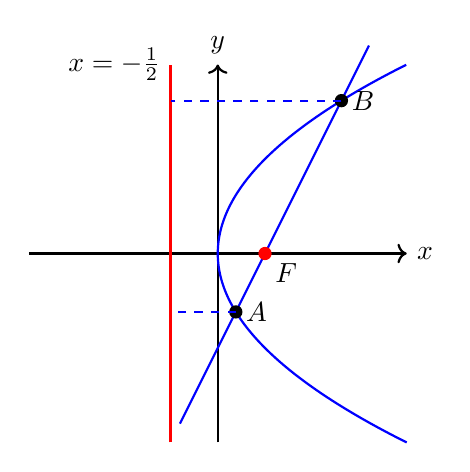
\begin{tikzpicture}[scale = 1.2,thick]
    % 定义参数 p 的值
    \def\p{1}
    \def\a{1} % 值和p 一样 ,解决 \p1=(intersection-1)  的冲突
    \def \t{1}
    \def \x{2}
    \def \y{2}
    \def \k{2}%定义斜率
    % 绘制坐标轴
    \draw[->,name=line3] (-\x,0) -- (\x,0) node[right] {$x$};
    \draw[->] (0,-\y) -- (0,\y) node[above] {$y$};
    % 绘制抛物线
    \draw[domain=-\t:\t, samples=100, smooth, variable=\t, blue,name path=Parabolic] plot ({2*\p*\t*\t}, {2*\p*\t});

    %准线图像
    \draw[red,name=line1] (-\p/2,-\y) -- (-\p/2,\y) node[left,black] {$x=-\frac{{\p}}{2}$};


    %交点弦
    \def \rate{0.9} %控制焦点弦的长参数,关于焦点对称
    \coordinate (M) at ($(\p/2,0)+{\rate+0.2}*(1,\k)$); 
    \coordinate (N) at ($(\p/2,0)-\rate*(1,\k)$); 

    \draw[blue, thick,name path=line]  (N) -- (M);%焦点弦

    \fill [ name intersections={of=line and Parabolic}]
    (intersection-1) circle (2pt) node[right] {$A$}
    (intersection-2) circle (2pt) node[right] {$B$};

    %焦点图像
    \coordinate (F) at (\p/2,0); %这个点是圆心
    \fill[red] (F) circle (2pt) node[below right,black] {$F$};


    % 3. 绘制虚线：将 \y 改为 A 的纵坐标（核心修改）
    \draw[dashed, blue] let \p1=(intersection-1) in % 提取 A 的坐标到 \p1
        (intersection-1) -- (-\a/2, \y1); % \y1 即 A 的纵坐标
    \draw[dashed, blue] let \p1=(intersection-2) in
        (intersection-2) -- (-\a/2, \y1);
\end{tikzpicture}
\end{document}

